\section{Overall structure of the proposed NoC-Architecture}

The proposed NoC architecture in Fig.~\ref{fig:System_Architecture} is designed to support three distinct Quality-of-Service (QoS) schemes in order to satisfy the heterogeneous communication requirements of different AXI4 masters and slaves:

\begin{figure}[htbp]
    \centering
    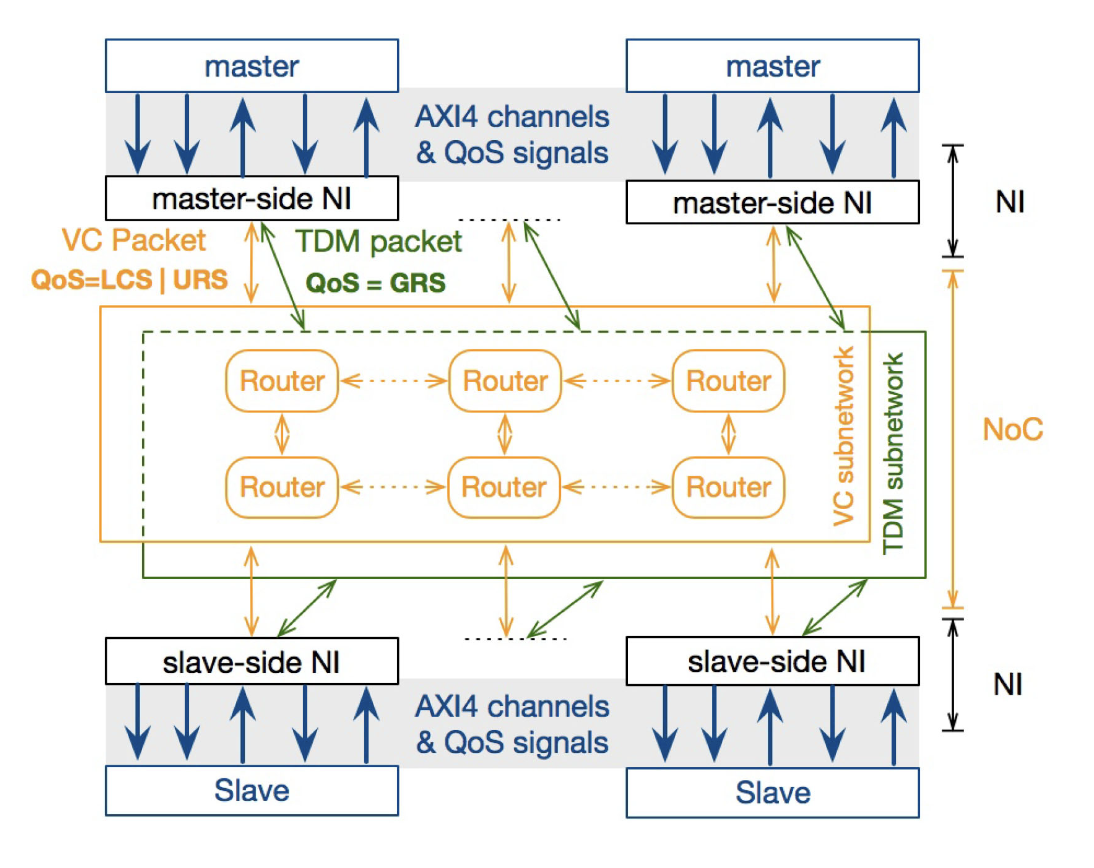
\includegraphics[width=0.95\textwidth]{img/System Architecture.png}
    \caption{System architecture\TODO{ar}}
    \label{fig:System_Architecture}
\end{figure}

\begin{itemize}
    \item \textbf{Latency-Critical Service (LCS):}\label{LCS} A low-latency forwarding service designed for bursty but non-streaming message transmissions. It provides fast delivery but does not guarantee bandwidth. Typical use cases include CPU-like masters that require short response times.
    \item \textbf{Guaranteed-Rate Service (GRS):}\label{GRS} A streaming service that ensures guaranteed bandwidth for large-volume data flows. It tolerates moderate latency but requires sustained throughput, as in GPU-like masters or other bandwidth-demanding accelerators.
    \item \textbf{Unspecified-Rate Service (URS):}\label{URS} A best-effort service that relies on currently available resources. It provides neither guaranteed bandwidth nor low latency, but aims at fairness among flows. URS is suitable for I/O interfaces such as SATA or USB.
\end{itemize}

To accommodate these QoS requirements, the system architecture is divided into three main components: (i) AXI4-based master/slave nodes, (ii) network interfaces (NIs) that perform protocol conversion and QoS mapping, and (iii) the NoC fabric itself, which consists of two subnetworks: a VC-based subnetwork for \ref{LCS} and \ref{URS} traffic, and a TDM-based subnetwork for \ref{GRS} traffic. 
This separation enables the NoC to meet diverse application needs without compromising performance or protocol compliance.
